\documentclass{report}

\usepackage[T2A]{fontenc}
\usepackage[russian]{babel}
\usepackage{graphicx}
\usepackage{float}
\usepackage{hyperref}
\usepackage{amsmath}
\usepackage{diffcoeff,amssymb}
\usepackage{mathtools}
\usepackage[normalem]{ulem}


%%%%%%%%%%%%%%%%%%%%%%%%%%%%%%%%%
% PACKAGE IMPORTS
%%%%%%%%%%%%%%%%%%%%%%%%%%%%%%%%%


\usepackage[tmargin=2cm,rmargin=1in,lmargin=1in,margin=0.85in,bmargin=2cm,footskip=.2in]{geometry}
\usepackage{amsmath,amsfonts,amsthm,amssymb,mathtools}
\usepackage[varbb]{newpxmath}
\usepackage{xfrac}
\usepackage[makeroom]{cancel}
\usepackage{mathtools}
\usepackage{bookmark}
\usepackage{enumitem}
\usepackage{hyperref,theoremref}
\hypersetup{
	pdftitle={Assignment},
	colorlinks=true, linkcolor=doc!90,
	bookmarksnumbered=true,
	bookmarksopen=true
}
\usepackage[most,many,breakable]{tcolorbox}
\usepackage{xcolor}
\usepackage{varwidth}
\usepackage{varwidth}
\usepackage{etoolbox}
%\usepackage{authblk}
\usepackage{nameref}
\usepackage{multicol,array}
\usepackage{tikz-cd}
\usepackage[ruled,vlined,linesnumbered]{algorithm2e}
\usepackage{comment} % enables the use of multi-line comments (\ifx \fi) 
\usepackage{import}
\usepackage{xifthen}
\usepackage{pdfpages}
\usepackage{transparent}

\newcommand\mycommfont[1]{\footnotesize\ttfamily\textcolor{blue}{#1}}
\SetCommentSty{mycommfont}
\newcommand{\incfig}[1]{%
    \def\svgwidth{\columnwidth}
    \import{./figures/}{#1.pdf_tex}
}

\usepackage{tikzsymbols}
\renewcommand\qedsymbol{$\Laughey$}


%\usepackage{import}
%\usepackage{xifthen}
%\usepackage{pdfpages}
%\usepackage{transparent}


%%%%%%%%%%%%%%%%%%%%%%%%%%%%%%
% SELF MADE COLORS
%%%%%%%%%%%%%%%%%%%%%%%%%%%%%%



\definecolor{myg}{RGB}{56, 140, 70}
\definecolor{myb}{RGB}{45, 111, 177}
\definecolor{myr}{RGB}{199, 68, 64}
\definecolor{mytheorembg}{HTML}{F2F2F9}
\definecolor{mytheoremfr}{HTML}{00007B}
\definecolor{mylenmabg}{HTML}{FFFAF8}
\definecolor{mylenmafr}{HTML}{983b0f}
\definecolor{mypropbg}{HTML}{f2fbfc}
\definecolor{mypropfr}{HTML}{191971}
\definecolor{myexamplebg}{HTML}{F2FBF8}
\definecolor{myexamplefr}{HTML}{88D6D1}
\definecolor{myexampleti}{HTML}{2A7F7F}
\definecolor{mydefinitbg}{HTML}{E5E5FF}
\definecolor{mydefinitfr}{HTML}{3F3FA3}
\definecolor{notesgreen}{RGB}{0,162,0}
\definecolor{myp}{RGB}{197, 92, 212}
\definecolor{mygr}{HTML}{2C3338}
\definecolor{myred}{RGB}{127,0,0}
\definecolor{myyellow}{RGB}{169,121,69}
\definecolor{myexercisebg}{HTML}{F2FBF8}
\definecolor{myexercisefg}{HTML}{88D6D1}


%%%%%%%%%%%%%%%%%%%%%%%%%%%%
% TCOLORBOX SETUPS
%%%%%%%%%%%%%%%%%%%%%%%%%%%%

\setlength{\parindent}{1cm}
%================================
% THEOREM BOX
%================================

\tcbuselibrary{theorems,skins,hooks}
\newtcbtheorem[number within=section]{Theorem}{Theorem}
{%
	enhanced,
	breakable,
	colback = mytheorembg,
	frame hidden,
	boxrule = 0sp,
	borderline west = {2pt}{0pt}{mytheoremfr},
	sharp corners,
	detach title,
	before upper = \tcbtitle\par\smallskip,
	coltitle = mytheoremfr,
	fonttitle = \bfseries\sffamily,
	description font = \mdseries,
	separator sign none,
	segmentation style={solid, mytheoremfr},
}
{th}

\tcbuselibrary{theorems,skins,hooks}
\newtcbtheorem[number within=chapter]{theorem}{Theorem}
{%
	enhanced,
	breakable,
	colback = mytheorembg,
	frame hidden,
	boxrule = 0sp,
	borderline west = {2pt}{0pt}{mytheoremfr},
	sharp corners,
	detach title,
	before upper = \tcbtitle\par\smallskip,
	coltitle = mytheoremfr,
	fonttitle = \bfseries\sffamily,
	description font = \mdseries,
	separator sign none,
	segmentation style={solid, mytheoremfr},
}
{th}


\tcbuselibrary{theorems,skins,hooks}
\newtcolorbox{Theoremcon}
{%
	enhanced
	,breakable
	,colback = mytheorembg
	,frame hidden
	,boxrule = 0sp
	,borderline west = {2pt}{0pt}{mytheoremfr}
	,sharp corners
	,description font = \mdseries
	,separator sign none
}

%================================
% Corollery
%================================
\tcbuselibrary{theorems,skins,hooks}
\newtcbtheorem[number within=section]{Corollary}{Corollary}
{%
	enhanced
	,breakable
	,colback = myp!10
	,frame hidden
	,boxrule = 0sp
	,borderline west = {2pt}{0pt}{myp!85!black}
	,sharp corners
	,detach title
	,before upper = \tcbtitle\par\smallskip
	,coltitle = myp!85!black
	,fonttitle = \bfseries\sffamily
	,description font = \mdseries
	,separator sign none
	,segmentation style={solid, myp!85!black}
}
{th}
\tcbuselibrary{theorems,skins,hooks}
\newtcbtheorem[number within=chapter]{corollary}{Corollary}
{%
	enhanced
	,breakable
	,colback = myp!10
	,frame hidden
	,boxrule = 0sp
	,borderline west = {2pt}{0pt}{myp!85!black}
	,sharp corners
	,detach title
	,before upper = \tcbtitle\par\smallskip
	,coltitle = myp!85!black
	,fonttitle = \bfseries\sffamily
	,description font = \mdseries
	,separator sign none
	,segmentation style={solid, myp!85!black}
}
{th}


%================================
% LENMA
%================================

\tcbuselibrary{theorems,skins,hooks}
\newtcbtheorem[number within=section]{Lenma}{Lenma}
{%
	enhanced,
	breakable,
	colback = mylenmabg,
	frame hidden,
	boxrule = 0sp,
	borderline west = {2pt}{0pt}{mylenmafr},
	sharp corners,
	detach title,
	before upper = \tcbtitle\par\smallskip,
	coltitle = mylenmafr,
	fonttitle = \bfseries\sffamily,
	description font = \mdseries,
	separator sign none,
	segmentation style={solid, mylenmafr},
}
{th}

\tcbuselibrary{theorems,skins,hooks}
\newtcbtheorem[number within=chapter]{lenma}{Lenma}
{%
	enhanced,
	breakable,
	colback = mylenmabg,
	frame hidden,
	boxrule = 0sp,
	borderline west = {2pt}{0pt}{mylenmafr},
	sharp corners,
	detach title,
	before upper = \tcbtitle\par\smallskip,
	coltitle = mylenmafr,
	fonttitle = \bfseries\sffamily,
	description font = \mdseries,
	separator sign none,
	segmentation style={solid, mylenmafr},
}
{th}


%================================
% PROPOSITION
%================================

\tcbuselibrary{theorems,skins,hooks}
\newtcbtheorem[number within=section]{Prop}{Proposition}
{%
	enhanced,
	breakable,
	colback = mypropbg,
	frame hidden,
	boxrule = 0sp,
	borderline west = {2pt}{0pt}{mypropfr},
	sharp corners,
	detach title,
	before upper = \tcbtitle\par\smallskip,
	coltitle = mypropfr,
	fonttitle = \bfseries\sffamily,
	description font = \mdseries,
	separator sign none,
	segmentation style={solid, mypropfr},
}
{th}

\tcbuselibrary{theorems,skins,hooks}
\newtcbtheorem[number within=chapter]{prop}{Proposition}
{%
	enhanced,
	breakable,
	colback = mypropbg,
	frame hidden,
	boxrule = 0sp,
	borderline west = {2pt}{0pt}{mypropfr},
	sharp corners,
	detach title,
	before upper = \tcbtitle\par\smallskip,
	coltitle = mypropfr,
	fonttitle = \bfseries\sffamily,
	description font = \mdseries,
	separator sign none,
	segmentation style={solid, mypropfr},
}
{th}


%================================
% CLAIM
%================================

\tcbuselibrary{theorems,skins,hooks}
\newtcbtheorem[number within=section]{claim}{Claim}
{%
	enhanced
	,breakable
	,colback = myg!10
	,frame hidden
	,boxrule = 0sp
	,borderline west = {2pt}{0pt}{myg}
	,sharp corners
	,detach title
	,before upper = \tcbtitle\par\smallskip
	,coltitle = myg!85!black
	,fonttitle = \bfseries\sffamily
	,description font = \mdseries
	,separator sign none
	,segmentation style={solid, myg!85!black}
}
{th}



%================================
% Exercise
%================================

\tcbuselibrary{theorems,skins,hooks}
\newtcbtheorem[number within=section]{Exercise}{Exercise}
{%
	enhanced,
	breakable,
	colback = myexercisebg,
	frame hidden,
	boxrule = 0sp,
	borderline west = {2pt}{0pt}{myexercisefg},
	sharp corners,
	detach title,
	before upper = \tcbtitle\par\smallskip,
	coltitle = myexercisefg,
	fonttitle = \bfseries\sffamily,
	description font = \mdseries,
	separator sign none,
	segmentation style={solid, myexercisefg},
}
{th}

\tcbuselibrary{theorems,skins,hooks}
\newtcbtheorem[number within=chapter]{exercise}{Exercise}
{%
	enhanced,
	breakable,
	colback = myexercisebg,
	frame hidden,
	boxrule = 0sp,
	borderline west = {2pt}{0pt}{myexercisefg},
	sharp corners,
	detach title,
	before upper = \tcbtitle\par\smallskip,
	coltitle = myexercisefg,
	fonttitle = \bfseries\sffamily,
	description font = \mdseries,
	separator sign none,
	segmentation style={solid, myexercisefg},
}
{th}

%================================
% EXAMPLE BOX
%================================

\newtcbtheorem[number within=section]{Example}{Example}
{%
	colback = myexamplebg
	,breakable
	,colframe = myexamplefr
	,coltitle = myexampleti
	,boxrule = 1pt
	,sharp corners
	,detach title
	,before upper=\tcbtitle\par\smallskip
	,fonttitle = \bfseries
	,description font = \mdseries
	,separator sign none
	,description delimiters parenthesis
}
{ex}

\newtcbtheorem[number within=chapter]{example}{Example}
{%
	colback = myexamplebg
	,breakable
	,colframe = myexamplefr
	,coltitle = myexampleti
	,boxrule = 1pt
	,sharp corners
	,detach title
	,before upper=\tcbtitle\par\smallskip
	,fonttitle = \bfseries
	,description font = \mdseries
	,separator sign none
	,description delimiters parenthesis
}
{ex}

%================================
% DEFINITION BOX
%================================

\newtcbtheorem[number within=section]{Definition}{Definition}{enhanced,
	before skip=2mm,after skip=2mm, colback=red!5,colframe=red!80!black,boxrule=0.5mm,
	attach boxed title to top left={xshift=1cm,yshift*=1mm-\tcboxedtitleheight}, varwidth boxed title*=-3cm,
	boxed title style={frame code={
					\path[fill=tcbcolback]
					([yshift=-1mm,xshift=-1mm]frame.north west)
					arc[start angle=0,end angle=180,radius=1mm]
					([yshift=-1mm,xshift=1mm]frame.north east)
					arc[start angle=180,end angle=0,radius=1mm];
					\path[left color=tcbcolback!60!black,right color=tcbcolback!60!black,
						middle color=tcbcolback!80!black]
					([xshift=-2mm]frame.north west) -- ([xshift=2mm]frame.north east)
					[rounded corners=1mm]-- ([xshift=1mm,yshift=-1mm]frame.north east)
					-- (frame.south east) -- (frame.south west)
					-- ([xshift=-1mm,yshift=-1mm]frame.north west)
					[sharp corners]-- cycle;
				},interior engine=empty,
		},
	fonttitle=\bfseries,
	title={#2},#1}{def}
\newtcbtheorem[number within=chapter]{definition}{Definition}{enhanced,
	before skip=2mm,after skip=2mm, colback=red!5,colframe=red!80!black,boxrule=0.5mm,
	attach boxed title to top left={xshift=1cm,yshift*=1mm-\tcboxedtitleheight}, varwidth boxed title*=-3cm,
	boxed title style={frame code={
					\path[fill=tcbcolback]
					([yshift=-1mm,xshift=-1mm]frame.north west)
					arc[start angle=0,end angle=180,radius=1mm]
					([yshift=-1mm,xshift=1mm]frame.north east)
					arc[start angle=180,end angle=0,radius=1mm];
					\path[left color=tcbcolback!60!black,right color=tcbcolback!60!black,
						middle color=tcbcolback!80!black]
					([xshift=-2mm]frame.north west) -- ([xshift=2mm]frame.north east)
					[rounded corners=1mm]-- ([xshift=1mm,yshift=-1mm]frame.north east)
					-- (frame.south east) -- (frame.south west)
					-- ([xshift=-1mm,yshift=-1mm]frame.north west)
					[sharp corners]-- cycle;
				},interior engine=empty,
		},
	fonttitle=\bfseries,
	title={#2},#1}{def}



%================================
% Solution BOX
%================================

\makeatletter
\newtcbtheorem{question}{Question}{enhanced,
	breakable,
	colback=white,
	colframe=myb!80!black,
	attach boxed title to top left={yshift*=-\tcboxedtitleheight},
	fonttitle=\bfseries,
	title={#2},
	boxed title size=title,
	boxed title style={%
			sharp corners,
			rounded corners=northwest,
			colback=tcbcolframe,
			boxrule=0pt,
		},
	underlay boxed title={%
			\path[fill=tcbcolframe] (title.south west)--(title.south east)
			to[out=0, in=180] ([xshift=5mm]title.east)--
			(title.center-|frame.east)
			[rounded corners=\kvtcb@arc] |-
			(frame.north) -| cycle;
		},
	#1
}{def}
\makeatother

%================================
% SOLUTION BOX
%================================

\makeatletter
\newtcolorbox{solution}{enhanced,
	breakable,
	colback=white,
	colframe=myg!80!black,
	attach boxed title to top left={yshift*=-\tcboxedtitleheight},
	title=Solution,
	boxed title size=title,
	boxed title style={%
			sharp corners,
			rounded corners=northwest,
			colback=tcbcolframe,
			boxrule=0pt,
		},
	underlay boxed title={%
			\path[fill=tcbcolframe] (title.south west)--(title.south east)
			to[out=0, in=180] ([xshift=5mm]title.east)--
			(title.center-|frame.east)
			[rounded corners=\kvtcb@arc] |-
			(frame.north) -| cycle;
		},
}
\makeatother

%================================
% Question BOX
%================================

\makeatletter
\newtcbtheorem{qstion}{Question}{enhanced,
	breakable,
	colback=white,
	colframe=mygr,
	attach boxed title to top left={yshift*=-\tcboxedtitleheight},
	fonttitle=\bfseries,
	title={#2},
	boxed title size=title,
	boxed title style={%
			sharp corners,
			rounded corners=northwest,
			colback=tcbcolframe,
			boxrule=0pt,
		},
	underlay boxed title={%
			\path[fill=tcbcolframe] (title.south west)--(title.south east)
			to[out=0, in=180] ([xshift=5mm]title.east)--
			(title.center-|frame.east)
			[rounded corners=\kvtcb@arc] |-
			(frame.north) -| cycle;
		},
	#1
}{def}
\makeatother

\newtcbtheorem[number within=chapter]{wconc}{Wrong Concept}{
	breakable,
	enhanced,
	colback=white,
	colframe=myr,
	arc=0pt,
	outer arc=0pt,
	fonttitle=\bfseries\sffamily\large,
	colbacktitle=myr,
	attach boxed title to top left={},
	boxed title style={
			enhanced,
			skin=enhancedfirst jigsaw,
			arc=3pt,
			bottom=0pt,
			interior style={fill=myr}
		},
	#1
}{def}



%================================
% NOTE BOX
%================================

\usetikzlibrary{arrows,calc,shadows.blur}
\tcbuselibrary{skins}
\newtcolorbox{note}[1][]{%
	enhanced jigsaw,
	colback=gray!20!white,%
	colframe=gray!80!black,
	size=small,
	boxrule=1pt,
	title=\textbf{Note:-},
	halign title=flush center,
	coltitle=black,
	breakable,
	drop shadow=black!50!white,
	attach boxed title to top left={xshift=1cm,yshift=-\tcboxedtitleheight/2,yshifttext=-\tcboxedtitleheight/2},
	minipage boxed title=1.5cm,
	boxed title style={%
			colback=white,
			size=fbox,
			boxrule=1pt,
			boxsep=2pt,
			underlay={%
					\coordinate (dotA) at ($(interior.west) + (-0.5pt,0)$);
					\coordinate (dotB) at ($(interior.east) + (0.5pt,0)$);
					\begin{scope}
						\clip (interior.north west) rectangle ([xshift=3ex]interior.east);
						\filldraw [white, blur shadow={shadow opacity=60, shadow yshift=-.75ex}, rounded corners=2pt] (interior.north west) rectangle (interior.south east);
					\end{scope}
					\begin{scope}[gray!80!black]
						\fill (dotA) circle (2pt);
						\fill (dotB) circle (2pt);
					\end{scope}
				},
		},
	#1,
}

%%%%%%%%%%%%%%%%%%%%%%%%%%%%%%
% SELF MADE COMMANDS
%%%%%%%%%%%%%%%%%%%%%%%%%%%%%%


\newcommand{\thm}[2]{\begin{Theorem}{#1}{}#2\end{Theorem}}
\newcommand{\cor}[2]{\begin{Corollary}{#1}{}#2\end{Corollary}}
\newcommand{\mlenma}[2]{\begin{Lenma}{#1}{}#2\end{Lenma}}
\newcommand{\mprop}[2]{\begin{Prop}{#1}{}#2\end{Prop}}
\newcommand{\clm}[3]{\begin{claim}{#1}{#2}#3\end{claim}}
\newcommand{\wc}[2]{\begin{wconc}{#1}{}\setlength{\parindent}{1cm}#2\end{wconc}}
\newcommand{\thmcon}[1]{\begin{Theoremcon}{#1}\end{Theoremcon}}
\newcommand{\ex}[2]{\begin{Example}{#1}{}#2\end{Example}}
\newcommand{\dfn}[2]{\begin{Definition}[colbacktitle=red!75!black]{#1}{}#2\end{Definition}}
\newcommand{\dfnc}[2]{\begin{definition}[colbacktitle=red!75!black]{#1}{}#2\end{definition}}
\newcommand{\qs}[2]{\begin{question}{#1}{}#2\end{question}}
\newcommand{\pf}[2]{\begin{myproof}[#1]#2\end{myproof}}
\newcommand{\nt}[1]{\begin{note}#1\end{note}}

\newcommand*\circled[1]{\tikz[baseline=(char.base)]{
		\node[shape=circle,draw,inner sep=1pt] (char) {#1};}}
\newcommand\getcurrentref[1]{%
	\ifnumequal{\value{#1}}{0}
	{??}
	{\the\value{#1}}%
}
\newcommand{\getCurrentSectionNumber}{\getcurrentref{section}}
\newenvironment{myproof}[1][\proofname]{%
	\proof[\bfseries #1: ]%
}{\endproof}

\newcommand{\mclm}[2]{\begin{myclaim}[#1]#2\end{myclaim}}
\newenvironment{myclaim}[1][\claimname]{\proof[\bfseries #1: ]}{}

\newcounter{mylabelcounter}

\makeatletter
\newcommand{\setword}[2]{%
	\phantomsection
	#1\def\@currentlabel{\unexpanded{#1}}\label{#2}%
}
\makeatother




\tikzset{
	symbol/.style={
			draw=none,
			every to/.append style={
					edge node={node [sloped, allow upside down, auto=false]{$#1$}}}
		}
}


% deliminators
\DeclarePairedDelimiter{\abs}{\lvert}{\rvert}
\DeclarePairedDelimiter{\norm}{\lVert}{\rVert}

\DeclarePairedDelimiter{\ceil}{\lceil}{\rceil}
\DeclarePairedDelimiter{\floor}{\lfloor}{\rfloor}
\DeclarePairedDelimiter{\round}{\lfloor}{\rceil}

\newsavebox\diffdbox
\newcommand{\slantedromand}{{\mathpalette\makesl{d}}}
\newcommand{\makesl}[2]{%
\begingroup
\sbox{\diffdbox}{$\mathsurround=0pt#1\mathrm{#2}$}%
\pdfsave
\pdfsetmatrix{1 0 0.2 1}%
\rlap{\usebox{\diffdbox}}%
\pdfrestore
\hskip\wd\diffdbox
\endgroup
}
\newcommand{\dd}[1][]{\ensuremath{\mathop{}\!\ifstrempty{#1}{%
\slantedromand\@ifnextchar^{\hspace{0.2ex}}{\hspace{0.1ex}}}%
{\slantedromand\hspace{0.2ex}^{#1}}}}
\ProvideDocumentCommand\dv{o m g}{%
  \ensuremath{%
    \IfValueTF{#3}{%
      \IfNoValueTF{#1}{%
        \frac{\dd #2}{\dd #3}%
      }{%
        \frac{\dd^{#1} #2}{\dd #3^{#1}}%
      }%
    }{%
      \IfNoValueTF{#1}{%
        \frac{\dd}{\dd #2}%
      }{%
        \frac{\dd^{#1}}{\dd #2^{#1}}%
      }%
    }%
  }%
}
\providecommand*{\pdv}[3][]{\frac{\partial^{#1}#2}{\partial#3^{#1}}}
%  - others
\DeclareMathOperator{\Lap}{\mathcal{L}}
\DeclareMathOperator{\Var}{Var} % varience
\DeclareMathOperator{\Cov}{Cov} % covarience
\DeclareMathOperator{\E}{E} % expected

% Since the amsthm package isn't loaded

% I prefer the slanted \leq
\let\oldleq\leq % save them in case they're every wanted
\let\oldgeq\geq
\renewcommand{\leq}{\leqslant}
\renewcommand{\geq}{\geqslant}

% % redefine matrix env to allow for alignment, use r as default
% \renewcommand*\env@matrix[1][r]{\hskip -\arraycolsep
%     \let\@ifnextchar\new@ifnextchar
%     \array{*\c@MaxMatrixCols #1}}


%\usepackage{framed}
%\usepackage{titletoc}
%\usepackage{etoolbox}
%\usepackage{lmodern}


%\patchcmd{\tableofcontents}{\contentsname}{\sffamily\contentsname}{}{}

%\renewenvironment{leftbar}
%{\def\FrameCommand{\hspace{6em}%
%		{\color{myyellow}\vrule width 2pt depth 6pt}\hspace{1em}}%
%	\MakeFramed{\parshape 1 0cm \dimexpr\textwidth-6em\relax\FrameRestore}\vskip2pt%
%}
%{\endMakeFramed}

%\titlecontents{chapter}
%[0em]{\vspace*{2\baselineskip}}
%{\parbox{4.5em}{%
%		\hfill\Huge\sffamily\bfseries\color{myred}\thecontentspage}%
%	\vspace*{-2.3\baselineskip}\leftbar\textsc{\small\chaptername~\thecontentslabel}\\\sffamily}
%{}{\endleftbar}
%\titlecontents{section}
%[8.4em]
%{\sffamily\contentslabel{3em}}{}{}
%{\hspace{0.5em}\nobreak\itshape\color{myred}\contentspage}
%\titlecontents{subsection}
%[8.4em]
%{\sffamily\contentslabel{3em}}{}{}  
%{\hspace{0.5em}\nobreak\itshape\color{myred}\contentspage}



%%%%%%%%%%%%%%%%%%%%%%%%%%%%%%%%%%%%%%%%%%%
% TABLE OF CONTENTS
%%%%%%%%%%%%%%%%%%%%%%%%%%%%%%%%%%%%%%%%%%%

\usepackage{tikz}
\definecolor{doc}{RGB}{0,60,110}
\usepackage{titletoc}
\contentsmargin{0cm}
\titlecontents{chapter}[3.7pc]
{\addvspace{30pt}%
	\begin{tikzpicture}[remember picture, overlay]%
		\draw[fill=doc!60,draw=doc!60] (-7,-.1) rectangle (-0.9,.5);%
		\pgftext[left,x=-3.5cm,y=0.2cm]{\color{white}\Large\sc\bfseries Chapter\ \thecontentslabel};%
	\end{tikzpicture}\color{doc!60}\large\sc\bfseries}%
{}
{}
{\;\titlerule\;\large\sc\bfseries Page \thecontentspage
	\begin{tikzpicture}[remember picture, overlay]
		\draw[fill=doc!60,draw=doc!60] (2pt,0) rectangle (4,0.1pt);
	\end{tikzpicture}}%
\titlecontents{section}[3.7pc]
{\addvspace{2pt}}
{\contentslabel[\thecontentslabel]{2pc}}
{}
{\hfill\small \thecontentspage}
[]
\titlecontents*{subsection}[3.7pc]
{\addvspace{-1pt}\small}
{}
{}
{\ --- \small\thecontentspage}
[ \textbullet\ ][]

\makeatletter
\renewcommand{\tableofcontents}{%
	\chapter*{%
	  \vspace*{-20\p@}%
	  \begin{tikzpicture}[remember picture, overlay]%
		  \pgftext[right,x=15cm,y=0.2cm]{\color{doc!60}\Huge\sc\bfseries \contentsname};%
		  \draw[fill=doc!60,draw=doc!60] (13,-.75) rectangle (20,1);%
		  \clip (13,-.75) rectangle (20,1);
		  \pgftext[right,x=15cm,y=0.2cm]{\color{white}\Huge\sc\bfseries \contentsname};%
	  \end{tikzpicture}}%
	\@starttoc{toc}}
\makeatother


%From M275 "Topology" at SJSU
\newcommand{\id}{\mathrm{id}}
\newcommand{\taking}[1]{\xrightarrow{#1}}
\newcommand{\inv}{^{-1}}

%From M170 "Introduction to Graph Theory" at SJSU
\DeclareMathOperator{\diam}{diam}
\DeclareMathOperator{\ord}{ord}
\newcommand{\defeq}{\overset{\mathrm{def}}{=}}

%From the USAMO .tex files
\newcommand{\ts}{\textsuperscript}
\newcommand{\dg}{^\circ}
\newcommand{\ii}{\item}

% % From Math 55 and Math 145 at Harvard
% \newenvironment{subproof}[1][Proof]{%
% \begin{proof}[#1] \renewcommand{\qedsymbol}{$\blacksquare$}}%
% {\end{proof}}

\newcommand{\liff}{\leftrightarrow}
\newcommand{\lthen}{\rightarrow}
\newcommand{\opname}{\operatorname}
\newcommand{\surjto}{\twoheadrightarrow}
\newcommand{\injto}{\hookrightarrow}
\newcommand{\On}{\mathrm{On}} % ordinals
\DeclareMathOperator{\img}{im} % Image
\DeclareMathOperator{\Img}{Im} % Image
\DeclareMathOperator{\coker}{coker} % Cokernel
\DeclareMathOperator{\Coker}{Coker} % Cokernel
\DeclareMathOperator{\Ker}{Ker} % Kernel
\DeclareMathOperator{\rank}{rank}
\DeclareMathOperator{\Spec}{Spec} % spectrum
\DeclareMathOperator{\Tr}{Tr} % trace
\DeclareMathOperator{\pr}{pr} % projection
\DeclareMathOperator{\ext}{ext} % extension
\DeclareMathOperator{\pred}{pred} % predecessor
\DeclareMathOperator{\dom}{dom} % domain
\DeclareMathOperator{\ran}{ran} % range
\DeclareMathOperator{\Hom}{Hom} % homomorphism
\DeclareMathOperator{\Mor}{Mor} % morphisms
\DeclareMathOperator{\End}{End} % endomorphism

\newcommand{\eps}{\epsilon}
\newcommand{\veps}{\varepsilon}
\newcommand{\ol}{\overline}
\newcommand{\ul}{\underline}
\newcommand{\wt}{\widetilde}
\newcommand{\wh}{\widehat}
\newcommand{\vocab}[1]{\textbf{\color{blue} #1}}
\providecommand{\half}{\frac{1}{2}}
\newcommand{\dang}{\measuredangle} %% Directed angle
\newcommand{\ray}[1]{\overrightarrow{#1}}
\newcommand{\seg}[1]{\overline{#1}}
\newcommand{\arc}[1]{\wideparen{#1}}
\DeclareMathOperator{\cis}{cis}
\DeclareMathOperator*{\lcm}{lcm}
\DeclareMathOperator*{\argmin}{arg min}
\DeclareMathOperator*{\argmax}{arg max}
\newcommand{\cycsum}{\sum_{\mathrm{cyc}}}
\newcommand{\symsum}{\sum_{\mathrm{sym}}}
\newcommand{\cycprod}{\prod_{\mathrm{cyc}}}
\newcommand{\symprod}{\prod_{\mathrm{sym}}}
\newcommand{\Qed}{\begin{flushright}\qed\end{flushright}}
\newcommand{\parinn}{\setlength{\parindent}{1cm}}
\newcommand{\parinf}{\setlength{\parindent}{0cm}}
% \newcommand{\norm}{\|\cdot\|}
\newcommand{\inorm}{\norm_{\infty}}
\newcommand{\opensets}{\{V_{\alpha}\}_{\alpha\in I}}
\newcommand{\oset}{V_{\alpha}}
\newcommand{\opset}[1]{V_{\alpha_{#1}}}
\newcommand{\lub}{\text{lub}}
\newcommand{\del}[2]{\frac{\partial #1}{\partial #2}}
\newcommand{\Del}[3]{\frac{\partial^{#1} #2}{\partial^{#1} #3}}
\newcommand{\deld}[2]{\dfrac{\partial #1}{\partial #2}}
\newcommand{\Deld}[3]{\dfrac{\partial^{#1} #2}{\partial^{#1} #3}}
\newcommand{\lm}{\lambda}
\newcommand{\uin}{\mathbin{\rotatebox[origin=c]{90}{$\in$}}}
\newcommand{\usubset}{\mathbin{\rotatebox[origin=c]{90}{$\subset$}}}
\newcommand{\lt}{\left}
\newcommand{\rt}{\right}
\newcommand{\bs}[1]{\boldsymbol{#1}}
\newcommand{\exs}{\exists}
\newcommand{\st}{\strut}
\newcommand{\dps}[1]{\displaystyle{#1}}

\newcommand{\sol}{\setlength{\parindent}{0cm}\textbf{\textit{Решение: }}\setlength{\parindent}{1cm} }
\newcommand{\solve}[1]{\setlength{\parindent}{0cm}\textbf{\textit{Решение: }}\setlength{\parindent}{1cm}#1 \Qed}

% Things Lie
\newcommand{\kb}{\mathfrak b}
\newcommand{\kg}{\mathfrak g}
\newcommand{\kh}{\mathfrak h}
\newcommand{\kn}{\mathfrak n}
\newcommand{\ku}{\mathfrak u}
\newcommand{\kz}{\mathfrak z}
\DeclareMathOperator{\Ext}{Ext} % Ext functor
\DeclareMathOperator{\Tor}{Tor} % Tor functor
\newcommand{\gl}{\opname{\mathfrak{gl}}} % frak gl group
\renewcommand{\sl}{\opname{\mathfrak{sl}}} % frak sl group chktex 6

% More script letters etc.
\newcommand{\SA}{\mathcal A}
\newcommand{\SB}{\mathcal B}
\newcommand{\SC}{\mathcal C}
\newcommand{\SF}{\mathcal F}
\newcommand{\SG}{\mathcal G}
\newcommand{\SH}{\mathcal H}
\newcommand{\OO}{\mathcal O}

\newcommand{\SCA}{\mathscr A}
\newcommand{\SCB}{\mathscr B}
\newcommand{\SCC}{\mathscr C}
\newcommand{\SCD}{\mathscr D}
\newcommand{\SCE}{\mathscr E}
\newcommand{\SCF}{\mathscr F}
\newcommand{\SCG}{\mathscr G}
\newcommand{\SCH}{\mathscr H}

% Mathfrak primes
\newcommand{\km}{\mathfrak m}
\newcommand{\kp}{\mathfrak p}
\newcommand{\kq}{\mathfrak q}

% number sets
\newcommand{\RR}[1][]{\ensuremath{\ifstrempty{#1}{\mathbb{R}}{\mathbb{R}^{#1}}}}
\newcommand{\NN}[1][]{\ensuremath{\ifstrempty{#1}{\mathbb{N}}{\mathbb{N}^{#1}}}}
\newcommand{\ZZ}[1][]{\ensuremath{\ifstrempty{#1}{\mathbb{Z}}{\mathbb{Z}^{#1}}}}
\newcommand{\QQ}[1][]{\ensuremath{\ifstrempty{#1}{\mathbb{Q}}{\mathbb{Q}^{#1}}}}
\newcommand{\CC}[1][]{\ensuremath{\ifstrempty{#1}{\mathbb{C}}{\mathbb{C}^{#1}}}}
\newcommand{\PP}[1][]{\ensuremath{\ifstrempty{#1}{\mathbb{P}}{\mathbb{P}^{#1}}}}
\newcommand{\HH}[1][]{\ensuremath{\ifstrempty{#1}{\mathbb{H}}{\mathbb{H}^{#1}}}}
\newcommand{\FF}[1][]{\ensuremath{\ifstrempty{#1}{\mathbb{F}}{\mathbb{F}^{#1}}}}
% expected value
\newcommand{\EE}{\ensuremath{\mathbb{E}}}
\newcommand{\charin}{\text{ char }}
\DeclareMathOperator{\sign}{sign}
\DeclareMathOperator{\Aut}{Aut}
\DeclareMathOperator{\Inn}{Inn}
\DeclareMathOperator{\Syl}{Syl}
\DeclareMathOperator{\Gal}{Gal}
\DeclareMathOperator{\GL}{GL} % General linear group
\DeclareMathOperator{\SL}{SL} % Special linear group

%---------------------------------------
% BlackBoard Math Fonts :-
%---------------------------------------

%Captital Letters
\newcommand{\bbA}{\mathbb{A}}	\newcommand{\bbB}{\mathbb{B}}
\newcommand{\bbC}{\mathbb{C}}	\newcommand{\bbD}{\mathbb{D}}
\newcommand{\bbE}{\mathbb{E}}	\newcommand{\bbF}{\mathbb{F}}
\newcommand{\bbG}{\mathbb{G}}	\newcommand{\bbH}{\mathbb{H}}
\newcommand{\bbI}{\mathbb{I}}	\newcommand{\bbJ}{\mathbb{J}}
\newcommand{\bbK}{\mathbb{K}}	\newcommand{\bbL}{\mathbb{L}}
\newcommand{\bbM}{\mathbb{M}}	\newcommand{\bbN}{\mathbb{N}}
\newcommand{\bbO}{\mathbb{O}}	\newcommand{\bbP}{\mathbb{P}}
\newcommand{\bbQ}{\mathbb{Q}}	\newcommand{\bbR}{\mathbb{R}}
\newcommand{\bbS}{\mathbb{S}}	\newcommand{\bbT}{\mathbb{T}}
\newcommand{\bbU}{\mathbb{U}}	\newcommand{\bbV}{\mathbb{V}}
\newcommand{\bbW}{\mathbb{W}}	\newcommand{\bbX}{\mathbb{X}}
\newcommand{\bbY}{\mathbb{Y}}	\newcommand{\bbZ}{\mathbb{Z}}

%---------------------------------------
% MathCal Fonts :-
%---------------------------------------

%Captital Letters
\newcommand{\mcA}{\mathcal{A}}	\newcommand{\mcB}{\mathcal{B}}
\newcommand{\mcC}{\mathcal{C}}	\newcommand{\mcD}{\mathcal{D}}
\newcommand{\mcE}{\mathcal{E}}	\newcommand{\mcF}{\mathcal{F}}
\newcommand{\mcG}{\mathcal{G}}	\newcommand{\mcH}{\mathcal{H}}
\newcommand{\mcI}{\mathcal{I}}	\newcommand{\mcJ}{\mathcal{J}}
\newcommand{\mcK}{\mathcal{K}}	\newcommand{\mcL}{\mathcal{L}}
\newcommand{\mcM}{\mathcal{M}}	\newcommand{\mcN}{\mathcal{N}}
\newcommand{\mcO}{\mathcal{O}}	\newcommand{\mcP}{\mathcal{P}}
\newcommand{\mcQ}{\mathcal{Q}}	\newcommand{\mcR}{\mathcal{R}}
\newcommand{\mcS}{\mathcal{S}}	\newcommand{\mcT}{\mathcal{T}}
\newcommand{\mcU}{\mathcal{U}}	\newcommand{\mcV}{\mathcal{V}}
\newcommand{\mcW}{\mathcal{W}}	\newcommand{\mcX}{\mathcal{X}}
\newcommand{\mcY}{\mathcal{Y}}	\newcommand{\mcZ}{\mathcal{Z}}


%---------------------------------------
% Bold Math Fonts :-
%---------------------------------------

%Captital Letters
\newcommand{\bmA}{\boldsymbol{A}}	\newcommand{\bmB}{\boldsymbol{B}}
\newcommand{\bmC}{\boldsymbol{C}}	\newcommand{\bmD}{\boldsymbol{D}}
\newcommand{\bmE}{\boldsymbol{E}}	\newcommand{\bmF}{\boldsymbol{F}}
\newcommand{\bmG}{\boldsymbol{G}}	\newcommand{\bmH}{\boldsymbol{H}}
\newcommand{\bmI}{\boldsymbol{I}}	\newcommand{\bmJ}{\boldsymbol{J}}
\newcommand{\bmK}{\boldsymbol{K}}	\newcommand{\bmL}{\boldsymbol{L}}
\newcommand{\bmM}{\boldsymbol{M}}	\newcommand{\bmN}{\boldsymbol{N}}
\newcommand{\bmO}{\boldsymbol{O}}	\newcommand{\bmP}{\boldsymbol{P}}
\newcommand{\bmQ}{\boldsymbol{Q}}	\newcommand{\bmR}{\boldsymbol{R}}
\newcommand{\bmS}{\boldsymbol{S}}	\newcommand{\bmT}{\boldsymbol{T}}
\newcommand{\bmU}{\boldsymbol{U}}	\newcommand{\bmV}{\boldsymbol{V}}
\newcommand{\bmW}{\boldsymbol{W}}	\newcommand{\bmX}{\boldsymbol{X}}
\newcommand{\bmY}{\boldsymbol{Y}}	\newcommand{\bmZ}{\boldsymbol{Z}}
%Small Letters
\newcommand{\bma}{\boldsymbol{a}}	\newcommand{\bmb}{\boldsymbol{b}}
\newcommand{\bmc}{\boldsymbol{c}}	\newcommand{\bmd}{\boldsymbol{d}}
\newcommand{\bme}{\boldsymbol{e}}	\newcommand{\bmf}{\boldsymbol{f}}
\newcommand{\bmg}{\boldsymbol{g}}	\newcommand{\bmh}{\boldsymbol{h}}
\newcommand{\bmi}{\boldsymbol{i}}	\newcommand{\bmj}{\boldsymbol{j}}
\newcommand{\bmk}{\boldsymbol{k}}	\newcommand{\bml}{\boldsymbol{l}}
\newcommand{\bmm}{\boldsymbol{m}}	\newcommand{\bmn}{\boldsymbol{n}}
\newcommand{\bmo}{\boldsymbol{o}}	\newcommand{\bmp}{\boldsymbol{p}}
\newcommand{\bmq}{\boldsymbol{q}}	\newcommand{\bmr}{\boldsymbol{r}}
\newcommand{\bms}{\boldsymbol{s}}	\newcommand{\bmt}{\boldsymbol{t}}
\newcommand{\bmu}{\boldsymbol{u}}	\newcommand{\bmv}{\boldsymbol{v}}
\newcommand{\bmw}{\boldsymbol{w}}	\newcommand{\bmx}{\boldsymbol{x}}
\newcommand{\bmy}{\boldsymbol{y}}	\newcommand{\bmz}{\boldsymbol{z}}

%---------------------------------------
% Scr Math Fonts :-
%---------------------------------------

\newcommand{\sA}{{\mathscr{A}}}   \newcommand{\sB}{{\mathscr{B}}}
\newcommand{\sC}{{\mathscr{C}}}   \newcommand{\sD}{{\mathscr{D}}}
\newcommand{\sE}{{\mathscr{E}}}   \newcommand{\sF}{{\mathscr{F}}}
\newcommand{\sG}{{\mathscr{G}}}   \newcommand{\sH}{{\mathscr{H}}}
\newcommand{\sI}{{\mathscr{I}}}   \newcommand{\sJ}{{\mathscr{J}}}
\newcommand{\sK}{{\mathscr{K}}}   \newcommand{\sL}{{\mathscr{L}}}
\newcommand{\sM}{{\mathscr{M}}}   \newcommand{\sN}{{\mathscr{N}}}
\newcommand{\sO}{{\mathscr{O}}}   \newcommand{\sP}{{\mathscr{P}}}
\newcommand{\sQ}{{\mathscr{Q}}}   \newcommand{\sR}{{\mathscr{R}}}
\newcommand{\sS}{{\mathscr{S}}}   \newcommand{\sT}{{\mathscr{T}}}
\newcommand{\sU}{{\mathscr{U}}}   \newcommand{\sV}{{\mathscr{V}}}
\newcommand{\sW}{{\mathscr{W}}}   \newcommand{\sX}{{\mathscr{X}}}
\newcommand{\sY}{{\mathscr{Y}}}   \newcommand{\sZ}{{\mathscr{Z}}}


%---------------------------------------
% Math Fraktur Font
%---------------------------------------

%Captital Letters
\newcommand{\mfA}{\mathfrak{A}}	\newcommand{\mfB}{\mathfrak{B}}
\newcommand{\mfC}{\mathfrak{C}}	\newcommand{\mfD}{\mathfrak{D}}
\newcommand{\mfE}{\mathfrak{E}}	\newcommand{\mfF}{\mathfrak{F}}
\newcommand{\mfG}{\mathfrak{G}}	\newcommand{\mfH}{\mathfrak{H}}
\newcommand{\mfI}{\mathfrak{I}}	\newcommand{\mfJ}{\mathfrak{J}}
\newcommand{\mfK}{\mathfrak{K}}	\newcommand{\mfL}{\mathfrak{L}}
\newcommand{\mfM}{\mathfrak{M}}	\newcommand{\mfN}{\mathfrak{N}}
\newcommand{\mfO}{\mathfrak{O}}	\newcommand{\mfP}{\mathfrak{P}}
\newcommand{\mfQ}{\mathfrak{Q}}	\newcommand{\mfR}{\mathfrak{R}}
\newcommand{\mfS}{\mathfrak{S}}	\newcommand{\mfT}{\mathfrak{T}}
\newcommand{\mfU}{\mathfrak{U}}	\newcommand{\mfV}{\mathfrak{V}}
\newcommand{\mfW}{\mathfrak{W}}	\newcommand{\mfX}{\mathfrak{X}}
\newcommand{\mfY}{\mathfrak{Y}}	\newcommand{\mfZ}{\mathfrak{Z}}
%Small Letters
\newcommand{\mfa}{\mathfrak{a}}	\newcommand{\mfb}{\mathfrak{b}}
\newcommand{\mfc}{\mathfrak{c}}	\newcommand{\mfd}{\mathfrak{d}}
\newcommand{\mfe}{\mathfrak{e}}	\newcommand{\mff}{\mathfrak{f}}
\newcommand{\mfg}{\mathfrak{g}}	\newcommand{\mfh}{\mathfrak{h}}
\newcommand{\mfi}{\mathfrak{i}}	\newcommand{\mfj}{\mathfrak{j}}
\newcommand{\mfk}{\mathfrak{k}}	\newcommand{\mfl}{\mathfrak{l}}
\newcommand{\mfm}{\mathfrak{m}}	\newcommand{\mfn}{\mathfrak{n}}
\newcommand{\mfo}{\mathfrak{o}}	\newcommand{\mfp}{\mathfrak{p}}
\newcommand{\mfq}{\mathfrak{q}}	\newcommand{\mfr}{\mathfrak{r}}
\newcommand{\mfs}{\mathfrak{s}}	\newcommand{\mft}{\mathfrak{t}}
\newcommand{\mfu}{\mathfrak{u}}	\newcommand{\mfv}{\mathfrak{v}}
\newcommand{\mfw}{\mathfrak{w}}	\newcommand{\mfx}{\mathfrak{x}}
\newcommand{\mfy}{\mathfrak{y}}	\newcommand{\mfz}{\mathfrak{z}}

\newcommand\smallO{
  \mathchoice
    {{\scriptstyle\mathcal{O}}}% \displaystyle
    {{\scriptstyle\mathcal{O}}}% \textstyle
    {{\scriptscriptstyle\mathcal{O}}}% \scriptstyle
    {\scalebox{.7}{$\scriptscriptstyle\mathcal{O}$}}%\scriptscriptstyle
  }


\title{\Huge{Матан инд}\\ Вариант №19(22)}

\author{\huge{Евгений Турчанин}}
\date{}
\begin{document}
\maketitle

\qs{}{
Доказать что:
$\dfrac{1^4}{1\cdot3}+\dfrac{2^4}{3\cdot5}+\mathellipsis+\dfrac{n^4}{(2n-1)\cdot(2n+1)}=\dfrac{n(n+1)(n^2+n+1)}{6(2n+1)}$
}
\sol
Докажем через индукцию:\\
\begin{enumerate}
	\item Покажем что для $n=1$ верно: \\ 
		\begin{equation*}
		\dfrac{1(1+1)(1^2+1+1)}{6(2+1)}=\dfrac{1}{3}
		\end{equation*}
		\begin{equation*}
		\dfrac{1^4}{1\cdot3}=\dfrac{1}{3}
		\end{equation*}
	\item Пусть верно для $n$ \\
	\item Тогда докажем, что верно для $n+1$:
		\begin{equation*}
			\underbrace{\dfrac{1^4}{1\cdot3}+\dfrac{2^4}{3\cdot5}+\mathellipsis+\dfrac{n^4}{(2n-1)\cdot(2n+1)}}_{\dfrac{n(n+1)(n^2+n+1)}{6(2n+1)}}+\dfrac{(n+1)^4}{(2n+1)\cdot(2n+3)} \Rightarrow
		\end{equation*}
		Нужно доказать, что:
		\begin{equation*}
		\dfrac{n(n+1)(n^2+n+1)}{6(2n+1)}+\dfrac{(n+1)^4}{(2n+1)\cdot(2n+3)} = 
		\dfrac{(n+1)(n+2)(n^2+3n+3)}{6(2n+3)}
		\end{equation*}
		\sout{Трудно не заметить, что так оно и есть}
		Давайте покажем, что это так:\\
		Сократим все на $n+1$ и приведем к общему знаменателю:
		\begin{equation*}
		\dfrac{n(2n+3)(n^2+n+1)}{6(2n+1)(2n+3)}+\dfrac{6(n+1)^3}{6(2n+1)\cdot(2n+3)} = 
		\dfrac{(2n+1)(n+2)(n^2+3n+3)}{6(2n+1)(2n+3)}
		\end{equation*}
		Сократим на знаменатели и раскроем скобки:
		\begin{equation*}
		2x^4+11x^3+23x^2+21x+6=2x^3+11x^2+23x+21+6 \Rightarrow
		\end{equation*}
		\begin{equation*}
		0=0
		\end{equation*}
		\begin{center}
			Ч.Т.Д.
		\end{center}

\end{enumerate}



\qs{}{
Доказать что:
\[ \sum_{k=1}^{k}\dfrac{1}{k^2} \leqslant 2 -\dfrac{1}{n}\]
}
\sol
Докажем опять \sout{двадцатьпять} через индукцию:\\
\begin{enumerate}
	\item Покажем что для $n=1$ верно: \\ 
		\begin{equation*}
			\dfrac{1}{1^2}=1
		\end{equation*}
		\begin{equation*}
			2-\dfrac{1}{1}=1
		\end{equation*}
	\item Пусть верно для $n$ \\
	\item Тогда докажем, что верно для $n+1$:\\
		Те нужно доказать что верно:
		\begin{equation*}
			\underbrace{\dfrac{1}{1^2}+\dfrac{1}{2^2}+\mathellipsis+\dfrac{1}{n^2}}_{\leqslant 2-\frac{1}{n}}+\dfrac{1}{(n+1)^2} \leqslant 2-\dfrac{1}{n+1}
		\end{equation*}
		Приведем к общему знаменателю:
		\begin{equation*}
			\dfrac{(2n-1)(n+1)^2+n}{(n+1)^2n} \leqslant \dfrac{(2n+1)(n+1)n}{(n+1)^2n}
		\end{equation*}
		Сократим на знаменатель:
		\begin{equation*}
			(2n-1)(n+1)^2+n\leqslant (2n+1)(n+1)n
		\end{equation*}
		Раскроем скобки:
		\begin{equation*}
			2n^3+4n^2+2n-n^2-2n-1+n\leqslant 2n^3+2n^2+n^2+n \Rightarrow
		\end{equation*}
		\begin{equation*}
			-1\leqslant 0
		\end{equation*}
		\begin{center}
			Ч.Т.Д.
		\end{center}

\end{enumerate}


\begin{center}
	\textbf{\Large{Момент когда меня сместили с 19 на 22 место}}
\end{center}
\hrulefill

\qs{}{
Доказать:
$(2n-1)!<n^{2n-1}, \; n \geq 2$

}
\sol
Докажем по мат. индукции:
\begin{enumerate}
	\item Покажем что для $n=2$ верно: \\
		\begin{equation*}
			(4-1)!<2^{4-1} \Rightarrow 6<8
		\end{equation*}

	\item Пусть верно для $n$ \\
	\item Докажем, что верно для $n+1$ \\
		\begin{equation*}
			(2n+1)!<(n+1)^{2n+1} \Rightarrow 2n(2n+1)n^{2n-1}<(n+1)^{2n+1} \Rightarrow 
		\end{equation*}
		\begin{equation*}
			4n^{2n+1}+2n^{2n}<n^{2n+1}+(n+1)^{2n}\cdot(2n+1)+(n+1)^{2n-1}\cdot n(2n+1)
		\end{equation*}
		Преобразуем правую часть:
		\begin{equation*}
			n^{2n+1}+(n+1)^{2n}\cdot(2n+1)+(n+1)^{2n-1}\cdot n(2n+1)>5n^{2n+1}+2n^{2n}
		\end{equation*}
		Тк
		\begin{equation*}
			4n^{2n+1}+2n^{2n}<5n^{2n+1}+2n^{2n}
		\end{equation*}
		\begin{center}
		\textbf{Ч.Т.Д.}
		\end{center}
\end{enumerate}

\qs{}{
$C_n^0-2C_n^1+3C_n^2+\ldots +(-1)^n(n+1)C_n^n$ = ?
}
\sol
\sout{Легко}Трудно не заметить что:\\

\begin{equation*}
C_n^0-2C_n^1+3C_n^2+\ldots+(-1)^n(n+1)C_n^n=(n+1)C_n^0-nC_n^1+(n-1)C_n^2+\ldots+(-1)^nC_n^n
\end{equation*}
\\
Тогда начальную сумму можно представить ввиде:
\begin{equation*}
\dfrac{n+1}{2}(C_n^0-C_n^1+(-1)^nC_n^2+\ldots+C_n^n)
\end{equation*}

\begin{equation*}
C_n^0-C_n^1+C_n^2+\ldots+(-1)^nC_n^n=(a+b)^n
\end{equation*}
\\
Такое равенство будет выполнятся при $a=1$ и $b=-1$(причем, очевидно что четность/нечетность $n$ не влияет), тогда искомая сумма будет равна:
\begin{equation*}
\dfrac{n+1}{2}0^n=0
\end{equation*}

\clm{}{}{\textbf{Ответ\sout{ственность}:}
$C_n^0-2C_n^1+3C_n^2+\ldots +(-1)^n(n+1)C_n^n=0$
}
\hfill

\qs{}{
Доказать:
\begin{enumerate}
	\item $\lim\limits_{n\to\infty} \dfrac{3n-3}{6n-4}=\dfrac{1}{2}$
	\item $\lim\limits_{n\to\infty} (3-\ln{(n+1)})=-\infty$
	\item $\lim\limits_{n\to\infty} ((-1)^n\cdot n^2-n)=\infty$
\end{enumerate}
}
\sol

\begin{enumerate}
	\itemОпределение предела:
		\begin{equation*}
			\forall \epsilon > 0 \: \exists n_0 \in \mathbb{N}: \forall n \geq n_0: |A-x_n|< \epsilon
		\end{equation*}
		Тогда чтобы доказать что $1/2$ является пределом, нужно показать что:
		\begin{equation*}
			\left|\dfrac{1}{2}-\dfrac{3n-3}{6n-4}\right|<\epsilon
		\end{equation*}
		Те что $\left|\dfrac{1}{2}-\dfrac{3n-3}{6n-4}\right|$ может быть сколь угодно малым, покажем это:
		\begin{equation*}
			\left|\dfrac{1}{2}-\dfrac{3n-3}{6n-4}\right|=\dfrac{1}{6n-4} - \text{эта дробь может быть сколь угодно малой из принципа Архимеда}
		\end{equation*}
		\begin{center}
			\textbf{Ч.Т.Д.}
		\end{center}
	\item Если пределом последовательности является $-\infty$, то не существует такого числа, которое \textit{подпирает} последовательность снизу и последовательность монотонно убывает. Запишем это в формальном виде:
		\begin{equation*}
			\forall M \enspace \exists x_{n_0} : \forall n \geq n_0: x_n< M
		\end{equation*}
		Докажем что для любого $M$ можно найти такой $x_{n_0}$, начиная с которого, все члены мешьше $M$:
		\begin{equation*}
			3-\ln(n+1)<M \Rightarrow n>e^{3-M}-1  \text{--- ну вот он, можно округлить до целых и прибавить 1}
		\end{equation*}
		Теперь покажем монотонность последовательности:
		\begin{equation*}
			x_{n+1}-x_n=3-\ln{(n+2)}-3+\ln{(n+1)}=\ln{\dfrac{n+1}{n+2}}<0 \Rightarrow \text{последовательность монотонно убывает}
		\end{equation*}
		Получаем что, последовательность монотонно убывает и не ограничена снизу
		\begin{center}
			\textbf{Ч.Т.Д.}
		\end{center}
	\item Если предел последовательност это $\infty$, то множество ее частичных пределов --- $\lbrace-\infty, \infty\rbrace$\\
	Тогда докажем, что $\pm \infty$ являются частичными пределами, и что других частичных пределов нету:
	\begin{enumerate}
		\item $n$ - четное $\Rightarrow$
			$\lim\limits_{n\to\infty} (n^2-n)=\lim\limits_{n\to\infty} n^2(1-1/n) \to \infty$

		\item $n$ - нечетное $\Rightarrow$
			$\lim\limits_{n\to\infty} (-n^2-n)=\lim\limits_{n\to\infty} -n^2(1+1/n) \to -\infty$
	\end{enumerate}
	Других частичных пределов нету, тк в подпоследовательность входит либо бесконечное число четных и нечетных, тогда предел --- $\infty$, либо конечное число четных/нечетных и бесконечное число нечетных/четных, тогда с какого-то номера в подпоследовательности не будет четных/нечетных чисел, тогда частичне пределы --- $\mp \infty$
	\begin{center}
		\textbf{Ч.Т.Д.}
	\end{center}
\end{enumerate}

\qs{}{
$
\begin{gathered}
	1)\lim_{n\to\infty}\frac{5n\sqrt[\leftroot{0}\uproot{2}4]{n^3-2n}+n\sqrt{n^2+2n+8}}{\sqrt[\leftroot{0}\uproot{2}3]{n^6-5n+4}-3n^2-5n}; 2) \lim_{n\to\infty}\frac{3^{2n-1}+2^{n+5}+4n^5}{n\sqrt{3n+5}-9^{n+3}}; \\
3) \lim_{n\to\infty}\left(\sqrt{4n^4+3n^2+5}-\sqrt{4n^4-6n^2-7}\right); 4) \lim_{n\to\infty}\sqrt[n]{3+\frac{4}{2n-7}}; \\
5) \lim_{n\to\infty}\left(\frac{7n+15}{9n+8}\right)^{3n}; 6) \lim_{n\to\infty}\left(\frac{6n-5}{6n+7}\right)^{3n}; 7) \lim_{n\to\infty}\frac{n^{2}-(n+1)!}{n!\cdot(n+4)+5^{n}}; \\
8) \lim_{n\to\infty}\sqrt[n]{3n^{2}+\frac{4}{2n-7}}; 9) \lim_{n\to\infty}\frac{\sqrt[\leftroot{0}\uproot{2}n]{2}-1}{\sqrt[\leftroot{0}\uproot{2}n]{8}-1}; 10) \lim_{n\to\infty}\frac{3+6+9+...+3n}{n^{2}+4}. 
\end{gathered}
$
}
\begin{enumerate}
	\item $
		\lim\limits_{n\to\infty}\dfrac{5n\sqrt[\leftroot{0}\uproot{2}4]{n^3-2n}+n\sqrt{n^2+2n+8}}{\sqrt[\leftroot{0}\uproot{2}3]{n^6-5n+4}-3n^2-5n}=\lim\limits_{n\to\infty}\dfrac{5\sqrt[\leftroot{0}\uproot{2}4]{n^3-2n}+n\sqrt{1+2/n+8/n^2}}{n\sqrt[\leftroot{0}\uproot{2}3]{1-5/n^5+4/n^6}-n(3+5/n)}=\\
		\\
		\lim\limits_{n\to\infty}\dfrac{n\sqrt{1+2/n+8/n^2}\left(\dfrac{5\sqrt[\leftroot{0}\uproot{2}4]{n^3-2n}}{n\sqrt{1+2/n+8/n^2}}+1\right)}{n\sqrt[\leftroot{0}\uproot{2}3]{1-5/n^5+4/n^6}-n(3+5/n)}=
		\lim\limits_{n\to\infty}\dfrac{\sqrt{1+2/n+8/n^2}\left(\dfrac{5\sqrt[\leftroot{0}\uproot{2}4]{n^3-2n}}{n\sqrt{1+2/n+8/n^2}}+1\right)}{\sqrt[\leftroot{0}\uproot{2}3]{1-5/n^5+4/n^6}-(3+5/n)}=\\
		\lim\limits_{n\to\infty}\dfrac{\sqrt{1+2/n+8/n^2}\left(\dfrac{5\sqrt[\leftroot{0}\uproot{2}4]{n^3-2n}}{n\sqrt{1+2/n+8/n^2}}+1\right)}{(3+5/n)\left(\dfrac{\sqrt[\leftroot{0}\uproot{2}3]{1-5/n^5+4/n^6}}{3+5/n}-1\right)}=\dfrac{1\cdot1}{3\cdot\left(\dfrac{1}{3}-1\right)}=-\dfrac{1}{2}
	$
	\item $
		\lim\limits_{n\to\infty}\dfrac{3^{2n-1}+2^{n+5}+4n^5}{n\sqrt{3n+5}-9^{n+3}}=\lim\limits_{n\to\infty}\dfrac{9^{n}/3+2^{n}\cdot32+4n^5}{n\sqrt{3n+5}-9^{n}\cdot729}=
		\lim\limits_{n\to\infty}\dfrac{9^{n}/3\left(1+\dfrac{2^{n}\cdot32}{9^n/3}+\dfrac{4n^5}{9^n/3}\right)}{9^{n}\cdot729\left(\dfrac{n\sqrt{3n+5}}{9^n\cdot729}-1\right)}=\dfrac{1/3\cdot1}{729\cdot-1}=-\dfrac{1}{2187}
	$
\item $
	\lim\limits_{n\to\infty}\sqrt{4n^4+3n^2+5}-\sqrt{4n^4-6n^2-7}=\lim\limits_{n\to\infty}\dfrac{9n^2+12}{\sqrt{4n^4+3n^2+5}+\sqrt{4n^4-6n^2-7}}=\\
	\lim\limits_{n\to\infty}\dfrac{9n^2+12}{2n^2\sqrt{1+3/4n^2+5/4n^4}\left(1+\dfrac{\sqrt{4n^4-6n^2-7}}{\sqrt{4n^4+3n^2+5}}\right)}=\lim\limits_{n\to\infty}\dfrac{9n^2+12}{2n^2\sqrt{1+3/4n^2+5/4n^4}\left(1+\sqrt{1+\dfrac{-9n^2-9}{4n^4+3n^2+5}}\right)}=\dfrac{9}{2\cdot(1+1)}=\dfrac{9}{4}
$
\item $
	\lim\limits_{n\to\infty}\sqrt[n]{3+\dfrac{4}{2n-7}}=1 \quad \text{тк корень из чего-то положительного(что растет медленее корня) $\to$ 1}
$
\item $
\lim\limits_{n\to\infty}\left(\dfrac{7n+15}{9n+8}\right)^{3n}=\lim\limits_{n\to\infty}\left(\dfrac{7(1+15/n)}{9(1+8/n)}\right)^{3n}=0
$
\item $
	\lim\limits_{n\to\infty}\left(\dfrac{6n-5}{6n+7}\right)^{3n}=\lim\limits_{n\to\infty}\left(1+\dfrac{-12}{6n+7}\right)^{3n}=\lim\limits_{n\to\infty}e^{\frac{-12}{6n+7}\cdot 3n}=e^{-6}
$
\item $
	\lim\limits_{n\to\infty}\dfrac{n^{2}-(n+1)!}{n!\cdot(n+4)+5^{n}}=\lim\limits_{n\to\infty}\dfrac{(n+1)!\left(\dfrac{n^2}{(n+1)!}-1\right)}{n!(n+4)\left(1+\dfrac{5^n}{n!(n+4)}\right)}=
\lim\limits_{n\to\infty}\dfrac{-(n+1)}{n+4}=-1
$
\item $
\lim\limits_{n\to\infty}\sqrt[n]{3n^{2}+\dfrac{4}{2n-7}}=1 \quad \text{по аналогии с 4}
$
\item $
	\lim\limits_{n\to\infty}\dfrac{\sqrt[\leftroot{0}\uproot{2}n]{2}-1}{\sqrt[\leftroot{0}\uproot{2}n]{8}-1} \quad \text{используя $\sqrt[\leftroot{0}\uproot{2}n]{a}\approx1+\dfrac{\ln a}{n}$ при $n \to \infty$} \Rightarrow
	\lim\limits_{n\to\infty}\dfrac{\sqrt[\leftroot{0}\uproot{2}n]{2}-1}{\sqrt[\leftroot{0}\uproot{2}n]{8}-1}=\dfrac{\ln 2}{\ln 8}
$
\item $
\lim\limits_{n\to\infty}\dfrac{3+6+9+...+3n}{n^{2}+4}=\lim\limits_{n\to\infty}\dfrac{3n(n+1)}{n^{2}+4}=\lim\limits_{n\to\infty}\dfrac{3n^2(1+3/n)}{n^{2}(1+4/n^2)}=3
$
\end{enumerate}
\clm{}{}{\textbf{Ответ:}
\begin{enumerate}
	\item $-\dfrac{1}{2}$
	\item $-\dfrac{1}{2187}$
	\item $\dfrac{9}{4}$
	\item 1
	\item 0
	\item $e^{-6}$
	\item -1
	\item 1
	\item $\dfrac{\ln 2}{\ln 8}$
	\item 3
\end{enumerate}
}

\qs{}{
	Найти $\sup x_n,\: \inf x_n,\: \varliminf\limits_{n\to\infty}x_n,\: \varlimsup\limits_{n\to\infty}x_n$\\
	$x_n=\dfrac{2n+1}{n}\arccos{(-1)^n}$
}
\sol
\parindent ДлДля начала рассмотрим последовательность при четных $n$:\\
\[
	x_n=\dfrac{2n+1}{n}\arccos{1}=0 \quad - \text{\sout{офигенная}хорошая подпоследовательность}
\]
Теперь рассмотрим при нечетных $n$:\\
\[
	x_n=\dfrac{2n+1}{n}\pi=2+\dfrac{1}{n}\pi\quad-  \text{понятно, что это убыв. подпоследовательность}
\]
Понятно, что других подпоследовательностей нету, тк в последовательности может быть 3 случая:
\begin{enumerate}
	\item Бесконечное количество четных и нечетных номеров, тогда такая подпоследовательность не сход, тк нельзя найти номер после которого $\varepsilon$ можно взять любым, тк при четных можно найти 0, а при нечетных найти >2
	\item При конечном количестве четных и бесконечном количестве нечетных, можно найти номер с которого будут только нечетные, те подпоследовательность сход к $2$
	\item По аналогии с 2, но подпоследовательность сход к 0
\end{enumerate}
Теперь мы готовы сказать, что $\sup x_n = 3\pi$, $\inf x_n = 0$, $\varliminf\limits_{n\to\infty}x_n = 0$, $\varlimsup\limits_{n\to\infty}x_n = 2$ --- из определения $\varlimsup\limits_{n\to\infty}x_n = \lim\limits_{n\to\infty}(\sup_{m\geq n}x_m)$
\clm{}{}{\textbf{Ответ:}
\begin{enumerate}
	\item $\sup x_n = 3\pi$
	\item $\inf x_n = 0$
	\item $\varliminf\limits_{n\to\infty}x_n = 0$
	\item $\varlimsup\limits_{n\to\infty}x_n = 2$
\end{enumerate}
}
\qs{}{
	Определить сходится ли последовательность:\\
	\begin{center}
	$x_n=x_{n-1}+\dfrac{1}{2^n}$
	\end{center}
}
\sol
По критерию Коши: Если последовательность фундаментальна т.е.
\begin{equation}
	\forall \varepsilon > 0 \: \exists n_0:\: \forall n \geq n_0 \:\exists p \quad |x_{n+p}-x_n|<\varepsilon
\end{equation}
То последовательность сходится, для нашей последовательности возьмем p=1:
\begin{equation}
	x_n+\dfrac{1}{2^{n+1}}-x_n=\dfrac{1}{2^{n+1}}
\end{equation}
Понятно, что $\dfrac{1}{2^{n+1}}$ может быть сколь угодно малым $\Rightarrow$ последовательность сходится

\qs{}{
Используя признак Вейерштрасса, доказать, что данная последовательность сходится, и найти ее предел\\
\begin{center}
$x_n=\dfrac{5}{2}\cdot\dfrac{9}{7}\cdot\dfrac{13}{12}...\dfrac{4n+1}{5n-3}$
\end{center}
}
\sol
Нашу последовательность можно переписать ввиде:
\begin{equation*}
	x_{n}=x_{n-1}\dfrac{4n+1}{5n-3}, \; n_1=\dfrac{5}{2}
\end{equation*}
Тогда покажем, что она огр. снизу и монотонно убывает:
\begin{equation*}
	\dfrac{x_n}{x_{n-1}}=\dfrac{4n+1}{5n-3}  \end{equation*}
Очевидно, что при $n>3$:
\begin{equation*}
\dfrac{4n+1}{5n-3}<1
\end{equation*}
Наша последовательность убывает, и очевидно она огр. снизу 0, тк каждый член получается путем, умножения положительных чисел
Тогда найдем предел:
\begin{equation*}
	A=A\cdot \dfrac{4n+1}{5n-3} \Rightarrow A=0
\end{equation*}
Те наша последовательность имеет предел 0
\clm{}{}{\textbf{Ответ:}
\\
\\
$x_n=\dfrac{5}{2}\cdot\dfrac{9}{7}\cdot\dfrac{13}{12}...\dfrac{4n+1}{5n-3}\to0$
}
\qs{}{
Найти сумму ряда:
\[
	\sum_{n=1}^{\infty}\dfrac{12}{4n^2-8n-5}
\]
}
\sol
Через метод неопределенных коэффициентов найдем разложение на две дроби:
\[
	\sum_{n=1}^{\infty}\dfrac{12}{(2n+1)(2n-5)}=\sum_{n=1}^{\infty}\dfrac{2}{2n-5}-\sum_{n=1}^{\infty}\dfrac{2}{2n+1}
\]
Трудно не заметить, что \[\sum_{n=1}^{\infty}\dfrac{2}{2n-5}=\sum_{n=2}^{\infty}\dfrac{2}{2n+1}=\sum_{n=1}^{\infty}\dfrac{2}{2n+1}-\dfrac{2}{3} \]
Тогда \[ \sum_{n=1}^{\infty}\dfrac{12}{4n^2-8n-5}=-\dfrac{2}{3}\]

\clm{}{}{\textbf{Ответ:}
\\
$\displaystyle \sum_{n=1}^{\infty}\dfrac{12}{4n^2-8n-5}=-\dfrac{2}{3}$

}


\qs{}{
Доказать по определению предела функции в точке (по Коши):
\[
	\lim\limits_{x\to1} \dfrac{5x^2-4x-1}{x-1}=6
\]
}
\sol
Из определения предела по Коши:
\begin{equation*}
\forall \varepsilon > 0 \enspace \exists \delta > 0: \forall x \in \mathbb{R}: \left| x-1\right|<\delta \Rightarrow \left|\dfrac{5x^2-4x-1}{x-1}-6\right|<\varepsilon
\end{equation*}
Раскроем модуль, тогда:
\begin{equation*}
\left|\dfrac{5x^2-4x-1}{x-1}-6\right|<\varepsilon \Rightarrow \left|\dfrac{5x^2-10x+5}{x-1}\right| \Rightarrow \left|x-1 \right|<\dfrac{\varepsilon}{5}
\end{equation*}
Понятно, что если мы возьмем $\delta=\dfrac{\varepsilon}{5}$, то все ок

\qs{}{
Доказать, что данный предел не существует:
\[
\lim\limits_{x\to +\infty} \tg x
\]
}
\sol
Чтобы показать, что предела не существует, нужно найти две последовательности, которые сходятся в разные точки:
\begin{equation*}
	x_{n_1}=\dfrac{\pi}{4}+\pi k, \enspace k \in \mathbb{Z} \quad \enspace
	x_{n_2}=\pi q, \enspace q \in \mathbb{Z}
\end{equation*}
Понятно, что $x_{n_1}$ идет к 1, а $x_{n_2}$ идет к 0, те \sout{беспредел} предела не существует

\qs{}{
Вычислить пределы:
\begin{enumerate}
\item $\lim\limits_{x\to1}\dfrac{\left(2x^{2}-x-1\right)^{2}}{x^{3}+2x^{2}-x-2}$
\item $\lim\limits_{x\to-8}\dfrac{10-x-6\sqrt{1-x}}{2+\sqrt[\leftroot{0}\uproot{2}3]{x}}$
\item $\lim\limits_{x\to\pi/4}\dfrac{\ln\mathrm{tg}x}{\cos2x}$
\item $\lim\limits_{x\to2}\dfrac{\ln\left(x-\sqrt[\leftroot{0}\uproot{2}3]{2x-3}\right)}{\sin\left(\pi x/2\right)-\sin\left[\left(x-1\right)\pi\right]}$
\item $\lim\limits_{x\to0}\left(1-\sin^2\dfrac{x}{2}\right)^{1/\ln\left(1+\mathrm{tg}^23x\right)}$
\item $\lim\limits_{x\to1\pm0}\left(\dfrac{2x-1}{x+1}\right)^{1/\left(\sqrt[\leftroot{0}\uproot{2}3]{x}-1\right)}$
\item $\lim\limits_{x\to\pi/4}\dfrac{\sqrt[\leftroot{0}\uproot{2}3]{\mathrm{tg}x}+(4x-\pi)\cos\dfrac{x}{4x-\pi}}{\lg\left(2+\mathrm{tg}x\right)}$
\item $\lim\limits_{x\to+0}\dfrac{\ln\left(1-\ln x\right)}{\ln\left(1-\lg x\right)}$
\end{enumerate}
}

\sol
\begin{enumerate}
\item
$
\lim\limits_{x\to1}\dfrac{\left(2x^{2}-x-1\right)^{2}}{x^{3}+2x^{2}-x-2}=\lim\limits_{x\to1}\dfrac{(2x+1)^2(x-1)}{(x+2)(x+1)}=0
$
\item
По правилу Лопиталя:\\
$
\lim\limits_{x\to-8}\dfrac{10-x-6\sqrt{1-x}}{2+\sqrt[\leftroot{0}\uproot{2}3]{x}}=\lim\limits_{x\to-8}\dfrac{-1+3/\sqrt{1-x}}{\dfrac{1}{3\sqrt[\leftroot{0}\uproot{2}3]{x^2}}}=0
$
\item
По правилу Лопиталя:\\
$
\lim\limits_{x\to\pi/4}\dfrac{\ln\mathrm{tg}x}{\cos2x}=\lim\limits_{x\to\pi/4}\dfrac{\dfrac{1}{\tg x}\cdot\dfrac{1}{\cos2x}}{-\sin 2x \cdot 2}=-1
$
\item
По правилу Лопиталя:\\
$
\lim\limits_{x\to2}\dfrac{\ln\left(x-\sqrt[\leftroot{0}\uproot{2}3]{2x-3}\right)}{\sin\left(\pi x/2\right)-\sin\left[\left(x-1\right)\pi\right]}=\lim\limits_{x\to2}\dfrac{\dfrac{1}{x-\sqrt[\leftroot{0}\uproot{2}3]{2x-3}}\cdot\left(1-\dfrac{1}{3}\cdot\dfrac{1}{2x-3}\cdot 2 \right)}{\cos\left({\dfrac{\pi x}{2}}\right)\pi/2-\cos((x-1)\pi)\pi}=\dfrac{2}{3\pi}
$
\item
$
\lim\limits_{x\to0}\left(1-\sin^2\dfrac{x}{2}\right)^{1/\ln\left(1+\mathrm{tg}^23x\right)}=\lim\limits_{x\to0}\exp\left[\dfrac{-\sin^2\dfrac{x}{2}}{\ln\left(1+\tg^2 3x\right)}\right]=
\lim\limits_{x\to0}\exp\left[\dfrac{-\sin(x/2)}{\dfrac{1}{1+\tg^2 3x}\cdot2\tg 3x\cdot\dfrac{1}{\cos^2 3x}\cdot 3}\right]=
$
\quad \\
$
=\lim\limits_{x\to0} \exp\left[\dfrac{-\sin x/2}{6\tg 3x}\right]=e^{-\dfrac{1}{36}}
$
\item
$
\lim\limits_{x\to1\pm0}\left(\dfrac{2x-1}{x+1}\right)^{1/\left(\sqrt[\leftroot{0}\uproot{2}3]{x}-1\right)}=\lim\limits_{x\to1\pm0} e^{\dfrac{\ln\left(\dfrac{2x-1}{x+1}\right)}{\sqrt[\leftroot{0}\uproot{2}3]{x}-1}}\Rightarrow
\lim\limits_{x\to1+0}\left(\dfrac{2x-1}{x+1}\right)^{1/\left(\sqrt[\leftroot{0}\uproot{2}3]{x}-1\right)}=0,\ \lim\limits_{x\to1-0}\left(\dfrac{2x-1}{x+1}\right)^{1/\left(\sqrt[\leftroot{0}\uproot{2}3]{x}-1\right)}=+\infty
$
\item
$
\lim\limits_{x\to\pi/4}\dfrac{\sqrt[\leftroot{0}\uproot{2}3]{\mathrm{tg}x}+(4x-\pi)\cos\dfrac{x}{4x-\pi}}{\lg\left(2+\mathrm{tg}x\right)},
$
\\
тк $\cos$ огр. можно на него \sout{положить} забить $\Rightarrow$
$
\lim\limits_{x\to\pi/4}\dfrac{\sqrt[\leftroot{0}\uproot{2}3]{\mathrm{tg}x}+(4x-\pi)\cos\dfrac{x}{4x-\pi}}{\lg\left(2+\mathrm{tg}x\right)}=
\lim\limits_{x\to\pi/4}\dfrac{\sqrt[\leftroot{0}\uproot{2}3]{\tg x}}{\lg(2+\tg x)}+\lim\limits_{x\to\pi/4}\dfrac{0}{\lg(2+\tg x)}=\dfrac{1}{\lg 3}
$
\item
$
\lim\limits_{x\to+0}\dfrac{\ln\left(1-\ln x\right)}{\ln\left(1-\lg x\right)}=\lim\limits_{x\to+0}\dfrac{\ln(\ln(e-x))}{\ln(\lg (10-x))}=1
$
\end{enumerate}


\qs{}{
\begin{enumerate}
\item
$x=\dfrac{t^2}{t-1},\ y=\dfrac{t^2-1}{t}$
\item $y=2+\left(x^2(2-x)\right)^{1/3}$
\item $y=\dfrac{x}{2}-\arctg x$
\end{enumerate}
}

\begin{enumerate}
\item
Для начала рассмотрим 'подозрительные' точки:\\
Если $t \to 1+0 \Rightarrow x\to +\infty, \ y\to 0$, если $t \to 1-0 \Rightarrow x\to -\infty, \ y\to 0$\\
Найдем асимптоты вида $y=kx+b \Rightarrow$ $k=\lim\limits_{t\to\pm\infty}\dfrac{y(t)}{x(t)}=\lim\limits_{t\to\pm\infty}\dfrac{t^3-t^2-t+1}{t^3}=1\text{,}\, b=\lim\limits_{t\to\pm\infty}y(t)-kx(t)=$\\
$=\lim\limits_{t\to\pm\infty}\dfrac{t^2-1}{t}-\dfrac{t^2}{t-1}=\lim\limits_{t\to\pm\infty}\dfrac{-t^2-t+1}{t^2-t}=-1 \Rightarrow y=x-1$\\
Получается, что:\\
$y=x-1$, $y=0$, $x=0$ - это асимптоты\\
Исследуем выражение на возрастание и убывание:\\
\[
	x'_t=\dfrac{t(t-2)}{(t-1)^2}\text{,}\quad
		y'_t=\dfrac{t^2+1}{t^2}\text{,}\quad
		y'_x=\dfrac{(t^2+1)(t-1)^2}{t^3(t-2)}\text{,}\quad
\]


\item ..




\item
График $\arctg x$ выглядит как график $\tg x$, но с перевернутыми осями, а $-\arctg x$ нужно еще отразить по горизонтали
\begin{figure}[H]
\center
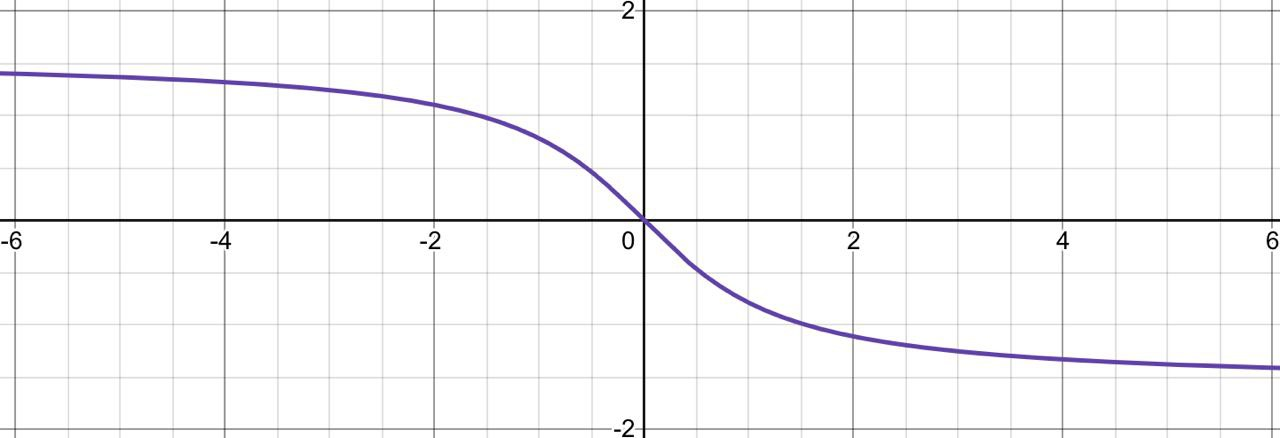
\includegraphics[width=0.5\textwidth]{pick_1}
\end{figure}
\end{enumerate}












\qs{}{
В куб с ребром $a$ вписан прямой круговой цилиндр так, что его ось совпадает с диагональю куба, а окружности оснований касаются граней куба. При каких размерах цилиндра его объем будет наибольшим?
}


\qs{}{
\begin{enumerate}
\item $\lim\limits_{x\to0}\dfrac{\left((1+3x)^{1/3}-1\right)/\tg x-\exp[-\sh x]-x^2(x+5)/(x+6)}{\ln \left(2\exp[x^2]-1\right)/\sin x-\arctg 2x}$
\item $\lim\limits_{x\to1}\left(\dfrac{1}{\ln x}-\dfrac{2}{x^2-1}\right)^{\dfrac{1}{\sin (x-1)}}$
\end{enumerate}
}

\begin{enumerate}
\item
Разложим слагаемые в ряд тейлора:\\

\begin{equation*}
\dfrac{(1+3x)^{1/3}-1}{\tg x}=\dfrac{x-x^2+\dfrac{5x^3}{3}}{x+\dfrac{x^3}{3}}+o(x^3)=\dfrac{3-3x+5x^2}{3+x^2}+o(x^3)\\
\end{equation*}

\begin{equation*}
\exp[-\sh x]=1-x-\dfrac{x^3}{6}+\dfrac{(-x-x^3/6)^2}{2}+\dfrac{(-x-x^3/6)^3}{6}=1-x+x^2/2-x^3/3+o(x^3)
\end{equation*}

\begin{equation*}
\dfrac{\ln \left(2\exp[x^2]-1\right)}{\sin x}=\dfrac{\ln(1+2x^2+x^4)}{x-x^3/6}+o(x^3)=\dfrac{2x^2+x^4-2x^4}{x-x^3/6}+o(x^3)=\dfrac{12x-6x^3}{6-x^2}+o(x^3)
\end{equation*}

\[
\arctg 2x=2x-\dfrac{8x^3}{3}+o(x^3)
\]

Подставляем всю эту гадостоть в уравнение:\\

\[
\lim\limits_{x\to0}\dfrac{\dfrac{3-3x+5x^2}{3+x^2}-\left(1-x+x^2/2-x^3/3\right)-x^2(x+5)/(x+6)}{\dfrac{12x-6x^3}{6-x^2}-2x+\dfrac{8x^3}{3}}+o(x^3)=\\
\lim\limits_{x\to0}\dfrac{\dfrac{2.5x^2+x^3}{3+x^2}-\dfrac{x^3+5x^2}{x+6}}{12x^3/(6-x^2)}+o(x^3)
\]

\[
\lim\limits_{x\to0}\dfrac{\dfrac{2.5x^3+15x^2+6x^3+3x^3-15x^2}{3x+18+x^3+6x^2}}{2x^3}+o(x^3)=\dfrac{23}{72}
\]

\item
Ну по аналогии \sout{упр}, заменим $t=x-1$

\[
\lim\limits_{t\to0}\left(\dfrac{1}{\ln (t+1)}-\dfrac{2}{t^2+2t}\right)^{\dfrac{1}{\sin t}}=
\lim\limits_{t\to0}\left(\dfrac{t^2+2t-2(t-t^2/2+t^3/3)}{(t^2+2t)(t-t^2)}\right)^{\dfrac{1}{\sin t}}
\lim\limits_{t\to0}\left(\dfrac{2t^2-2/3t^3}{2t^2}\right)^{\dfrac{1}{\sin t}}=
\]
\[
\lim\limits_{t\to0}\left( 1-1/3t\right)^{\dfrac{1}{\sin t}}=e^{\dfrac{1}{\sin t}\cdot-\dfrac{t}{3}}=e^{-1/3}
\]
\end{enumerate}



\end{document}
